%% filename: amsart-template.tex
%% version: 1.1
%% date: 2014/07/24
%%
%% American Mathematical Society
%% Technical Support
%% Publications Technical Group
%% 201 Charles Street
%% Providence, RI 02904
%% USA
%% tel: (401) 455-4080
%%      (800) 321-4267 (USA and Canada only)
%% fax: (401) 331-3842
%% email: tech-support@ams.org
%% 
%% Copyright 2008-2010, 2014 American Mathematical Society.
%% 
%% This work may be distributed and/or modified under the
%% conditions of the LaTeX Project Public License, either version 1.3c
%% of this license or (at your option) any later version.
%% The latest version of this license is in
%%   http://www.latex-project.org/lppl.txt
%% and version 1.3c or later is part of all distributions of LaTeX
%% version 2005/12/01 or later.
%% 
%% This work has the LPPL maintenance status `maintained'.
%% 
%% The Current Maintainer of this work is the American Mathematical
%% Society.
%%
%% ====================================================================

%     AMS-LaTeX v.2 template for use with amsart
%
%     Remove any commented or uncommented macros you do not use.

\documentclass{amsart}

\newtheorem{theorem}{Theorem}[section]
\newtheorem{lemma}[theorem]{Lemma}
%\newcommand{\qp}[1]{\left(#1\right)}
%\newcommand{\qb}[1]{\left[#1\right]}
%\newcommand{\w}{\omega}
%\newcommand{\W}{\Omega}

\theoremstyle{definition}
\newtheorem{definition}[theorem]{Definition}
\newtheorem{example}[theorem]{Example}
\newtheorem{xca}[theorem]{Exercise}

\theoremstyle{remark}
\newtheorem{remark}[theorem]{Remark}

\numberwithin{equation}{section}
\usepackage{tristan}
\usepackage{pgfplots}  
\begin{document}

\title{Numerical discretisation of the thin-film problem}

%    Remove any unused author tags.

%    author one information
\author{Georgios Sialounas}
\address{}
\curraddr{}
\email{georgios.sialounas@hotmail.com}
\thanks{Tristan Pryer, Alex Lukyanov}

%    author two information
\author{}
\address{}
\curraddr{}
\email{}
\thanks{}

\subjclass[2010]{Primary }

\keywords{}

\date{}

\dedicatory{}

\begin{abstract}
	Notes on parameters and numerical discretisation of the thin-film approximation of flow in an oil layer on the deep sea surface. In one spatial dimension with periodic boundary conditions.
\end{abstract}

\maketitle

\section{Introduction}
In this report we describe the numerical discretisation aspects for thin film approximation of the spreading of oil layers on the deep sea surface at arbitrary Reynolds number, $Re$.  In this problem, the choice of  The rest of the report  Specifically, we describe the numerical discretisation we use for the PDE and of the domain.  


\section{Preliminaries}

\begin{Defn}[One-dimensional system of balance laws] We consider problems of the form 
	\begin{equation}\label{eq:1d_gen_balance_law_system}
	\begin{aligned}
	\vec{u}_t+\partial_x\vec{f \qp{\vec{p}; \vec{u}}}&=\vec{g}\qp{\vec p;\vec u},\\
	\vec{u}\qp{x,0}&=\vec{u}_0\qp{x},
	\end{aligned}\quad \text{ for } \qp{x,t}\in \W\times\qp{0,\infty}
	\end{equation}
	with $\vec{u}=\qp{u_1,\dots,u_m}^T$, $\vec{g}\qp{\vec{p}; \vec{u}}=\qp{g_1\qp{\vec{p};\vec{u}},\dots,g_m\qp{\vec{p};\vec{u}}}^T$ and $\vec{f}\qp{\vec{p}; \vec{u}}=\qp{f_1\qp{\vec{p};\vec{u}},\dots,f_m\qp{\vec{p};\vec{u}}}^T$ and complemented with periodic boundary conditions.
	In particular,
	\begin{equation}
	\dfunkmapsto{\vec{u}}{\mathbb{R}\times\mathbb{R}^+}{\mathbb{R}^m}{\qp{x,t}}{\vec{u}\qp{x,t}},
	\end{equation}
	the forcing function $\vec{g}$
	\begin{equation}
	\dfunkmapsto{\vec{g}}{\mathbb{R}^m}{\mathbb{R}^m}{\vec p\qp{x,t}, \vec{u}\qp{x,t}}{\vec{g}\qp{\vec p; \vec{u}\qp{x,t}}}
	\end{equation}
	the flux function $\vec{f}$
	\begin{equation}
	\dfunkmapsto{\vec{f}}{\mathbb{R}^m}{\mathbb{R}^m}{\vec p\qp {x,t}, \vec{u}\qp{x,t}}{\vec{f}\qp{\vec p; \vec{u}\qp{x,t}}}
	\end{equation}
	and the vector $\vec{p}$ is a parameter vector which is assumed to be known and prescribed. 
\end{Defn}

We will introduce all the parameters included in $\vec{p}$ here and quote their values. The  vector $\vec k$ of wavenumbers is given by
\begin{equation}
\vec{k}:=\pi\qb{-1,1,-3,3,-5,5,-7,7,-9,9}^T,
\end{equation}
and $B_j$ (see \ref{eq:B_V}) given by 
\begin{equation}
B_j:= \bracegs{\frac{4}{5}U\left([0,1]\right)}_{j=1}^{10}
\end{equation}
The angular frequency $\w$ is given by 
\begin{equation}
\w_j :=\pi \sqrt{\frac{100}{\pi}\abs {k_j}}.
\end{equation}
The reader should note that the reason for scaling $\vec{k}$ and $\vec{w}$ by $\pi$ is to  facilitate  periodicity with trigonometric forcing.
\begin{Rem} Note that we use an additional  set of parameters to run a second set of numerical experiments where we investigate the effect of increasing $k_j$ and $B_j$ (in (\ref{eq:B_V})) individually on $\min(h)$.  In this second set of parameters we use
	\begin{equation}\label{eq:second_parameter_set}
\begin{aligned}
{k}_j&:=2^j\pi,\quad, j=0,\dots,5\\
\w_j &:=\pi \sqrt{\frac{100}{\pi}\abs {k_j}}\\
B_j&:=\frac{1}{4}2^j,\quad j = 0,\dots,5.
\end{aligned}
	\end{equation}
\end{Rem}

\section{The Problem}
In one spatial dimension for $Re\approx 1$ when surface tension effects are neglected, the problem become
\begin{equation}
\begin{aligned}
\frac{\partial h}{\partial t} + \frac{\partial q}{\partial x}&=0\\
\frac{\partial q}{\partial t} + \frac{\partial }{\partial x}\qp{\frac{6}{5}\frac{q^2}{h}=\frac{2}{5}qV-\frac{1}{5}V^2h+Ka\frac{h^2}{2}}&=-Kah\frac{\partial B}{\partial x}-\frac{3}{Re}\frac{\qp{q-Vh}}{h^2},
\end{aligned}
\end{equation}
 complemented with periodic boundary conditions. We consider the problem in the spatial domain $\W:=\qb{-1,1}$ and the temporal domain $\qb{0,T}$. Functions V and B are due to the water wave motion and are assumed to be given.  In deep water conditions they are linear combinations of harmonic components with frequency $\w_j$ and the wave number $k_j$ and phase $\phi_j$.
 \begin{equation}\label{eq:B_V}
\begin{aligned}
B&=\sum_jB_j\sin{k_j-\w_jt-\phi_j}\\
V&=\sum_jB_j\delta\w_j\sin{k_j-\w_jt-\phi_j}.
\end{aligned}
 \end{equation}
We note that we are using periodic boundary conditions.  Lastly, the parameter $\delta$ is set at $10^{-3}$.
\section{Numerical Discretisation}
In this section we present the spatial and temporal discretisations we will use to approximate (\ref{eq:1d_gen_balance_law_system}).   We will use boldface notation for  vector-valued quantities in order to distinguish them from scalar quantities.  Firstly, we will introduce conventions for discretisation of the derivative of flux function, $\vec{f}$.  Then, we will present the temporal and spatial discretisation schemes.  

Briefly, we will use an Strong Stability Preserving Runge Kutta method for the temporal discretisation and a Weighted Essentially Non-Oscillatory scheme for the spatial discretisation.  

Briefly, Essentially Non Oscillatory (ENO) and Weighted Essentially Non-Oscillatory schemes have been used with success in a number of applications (cf. \cite{jiang1996efficient}, \cite{shu1998essentially}), including conservation laws and balance laws (see e.g. \cite{shu2020essentially} for an overview).  

They have several features which contributed to their widespread success.  These include a mechanism of computational stencil construction that can achieve arbitrarily high accuracy in regions where the solution is smooth, essentially non-oscillatory behaviour in the vicinity of discontinuities (no artificial, numerical overshoots and undershoots) and proven ability to simulate complex smooth solution structures (see \cite{shu1998essentially} for more details).  In the present work we only consider WENO schemes.

\subsection{Domain discretisation}
We partition the domain $\W=\qb{-1,1}$ uniformly by choosing points $-1=x_0<\dots<x_M=1$ and we denote the step-size by $h$.  We denote by $I_j$ the sub-interval $\qb{x_j,x_{j+1}}$ of $\W$, $j=0,\dots,M-1$.  In the temporal variable we partition the interval $\qb{0,T}$ into sub-intervals with end-points $0=t^0<\dots<t^N=T$, where $N$ is chosen such that a CFL condition is satisfied. We denote by $\vec u^n_j:=\vec u\qp{t^n,x_j}$ the exact solution to (\ref{eq:1d_gen_balance_law_system}) and by $\vec U^n_j$ we denote the approximation to $\vec u^n_j$, obtained by the chosen numerical scheme.



\subsection{Spatial discretisation}
We will denote by $\vec{U}^n_j$ the numerical approximation to $\vec u\qp{x_j, t^n}$.  
It is well known that numerical schemes for
non-linear conservation laws may converge to functions which are not weak-solutions of the original problem (see \cite[\S12.1]{leveque1992numerical}). We address this problem by expressing the method in conservation form. We use a consistent numerical flux
function $\vec{F}$, which takes $p+q+1$ arguments:
\begin{equation}\label{eq_defn_num_flux}
\dfunkmapstonumflux{\qp{\vec{U}^n_{j-p+1},\cdots,\vec{U}^n_{j+q}}}{\vec{F}^n_j}{{\vec{F}}\qp{\vec{U}^n_{j-p},\cdots,\vec{U}^n_{j+q}}}{\vec{F}\qp{\vec{v},\cdots,\vec{v}}}{\vec{f}\qp{\vec{v}}, }
\end{equation}
where $p$ and $q$ are simply used to determine the width of the
computational stencil.  We use $\vec{F}$ to approximate
$\partial_{x}\vec{f}$ such that
\begin{equation}\label{eq_num_approx_f}
\partial_{x}\vec{f}\qp{\vec{u}}\approx \frac{1}{h}\qp{{\vec{F}\qp{\vec{U}^n_{j-p},\cdots,\vec{U}^n_{j+q}}}-{\vec{F}\qp{\vec{U}^n_{j-p-1},\cdots,\vec{U}^n_{j+q-1}}}}.
\end{equation}
We can then use a method-of-lines approach in the discretisation of
(\ref{eq:1d_gen_balance_law_system}) by requiring
\begin{equation}\label{eq:method_of_lines_balance}
\frac{\mathrm{d}}{\mathrm{d}t}\vec{U}_j =  \frac{1}{h}\qp{{\vec{F}\qp{\vec{U}^n_{j-p},\cdots,\vec{U}^n_{j+q}}}-{\vec{F}\qp{\vec{U}^n_{j-p-1},\cdots,\vec{U}^n_{j+q-1}}}} \Foreach j=0, \dots, M.
\end{equation}


\subsection{Temporal discretisation}
We discretise the temporal derivative in the left-hand side of (\ref{eq:method_of_lines_balance}) using a third order  Strong-Stability-Preserving Runge-Kutta (SSP3-RK) method.  We provide this as a Butcher tableaux:
\begin{equation}\label{defn:SSP3-temp}
\begin{array}{c|ccc}0&0&0&0\\1&1&0&0\\1/2&1/4&1/4&0\\\hline &1/6&1/6&2/3\\\end{array}
\end{equation} 

\subsection{Third order WENO scheme}
The WENO scheme consists of a procedure (the WENO Reconstruction procedure) which yields a difference quotient based on a wide computational stencil.  This procedure ensures the high order accuracy in areas where the solution is smooth and the non-oscillatory behaviour across discontinuities.  The details of the procedure are omitted here for the sake of brevity.  

In one spatial dimension, the WENO reconstruction procedure for the third order finite difference WENO scheme is used to approximate the components of the flux function $\vec{f}_x$, namely the $ {f_j}_x$, on the cell $I_j:=\qb{x_j, x_{j+1}}$.  The cell $I_j$ is chosen to be the central cell of the computational stencil $S:=\bracegs{I_{j-1}, I_j, I_{j+1}}$.  The approximation is then obtained as a convex combination of polynomials over two sub-stencils of $S$, namely 
\begin{equation}
\begin{aligned}
S_1&:=\bracegs{I_{j-1}, I_j}\quad \text{and}\\
S_2&:=\bracegs{I_{j}, I_{j+1}}.
\end{aligned}
\end{equation}
The next step is to derive polynomials, $p_1\qp{x}$and
$p_2\qp{x}$ which are the ENO reconstructions of $\vec f$
on the substencils $S_1$ and $S_2$
respectively.  The numerical flux at $x_{j}$, denoted by
$F_{j}$, is obtained as the combination
\begin{equation}\label{eq_f_WENO}
F_{j}:=w_1p_1\qp{x_{j}} +w_2p_2\qp{x_{j}},
\end{equation}
where $w_1$ and $w_2$ are the non-linear weights (see \cite{shu1998essentially} for more information on obtaining non-linear weights) corresponding to $S_1$and $S_2$, which have to satisfy the conditions
\begin{equation}
w_l\geq 0,\quad \sum_{l=1}^2 w_l = 1.
\end{equation}
Finally, the WENO approximation to the flux derivative is obtained using
\begin{equation}\label{eq_WENO_approx_flux_derivative}
\partial_x f_j\approx \frac{1}{h_{j-1}}\qp{F_{j}- F_{j-1}}.
\end{equation}
The reader should note that we have omitted all details pertaining to flux construction and derivation of weights. 
\section{Numerical Results}
In this section we present the numerical results using the parameters we described in (\ref{eq:second_parameter_set}).  We note that the forcing is not a single trigonometric function but rather the right hand side that results from the analysis in the thin film paper. The results are shown in Fig. \ref{fig:effect_Bj_kj_minh}

\begin{figure}[h]
	\centering
	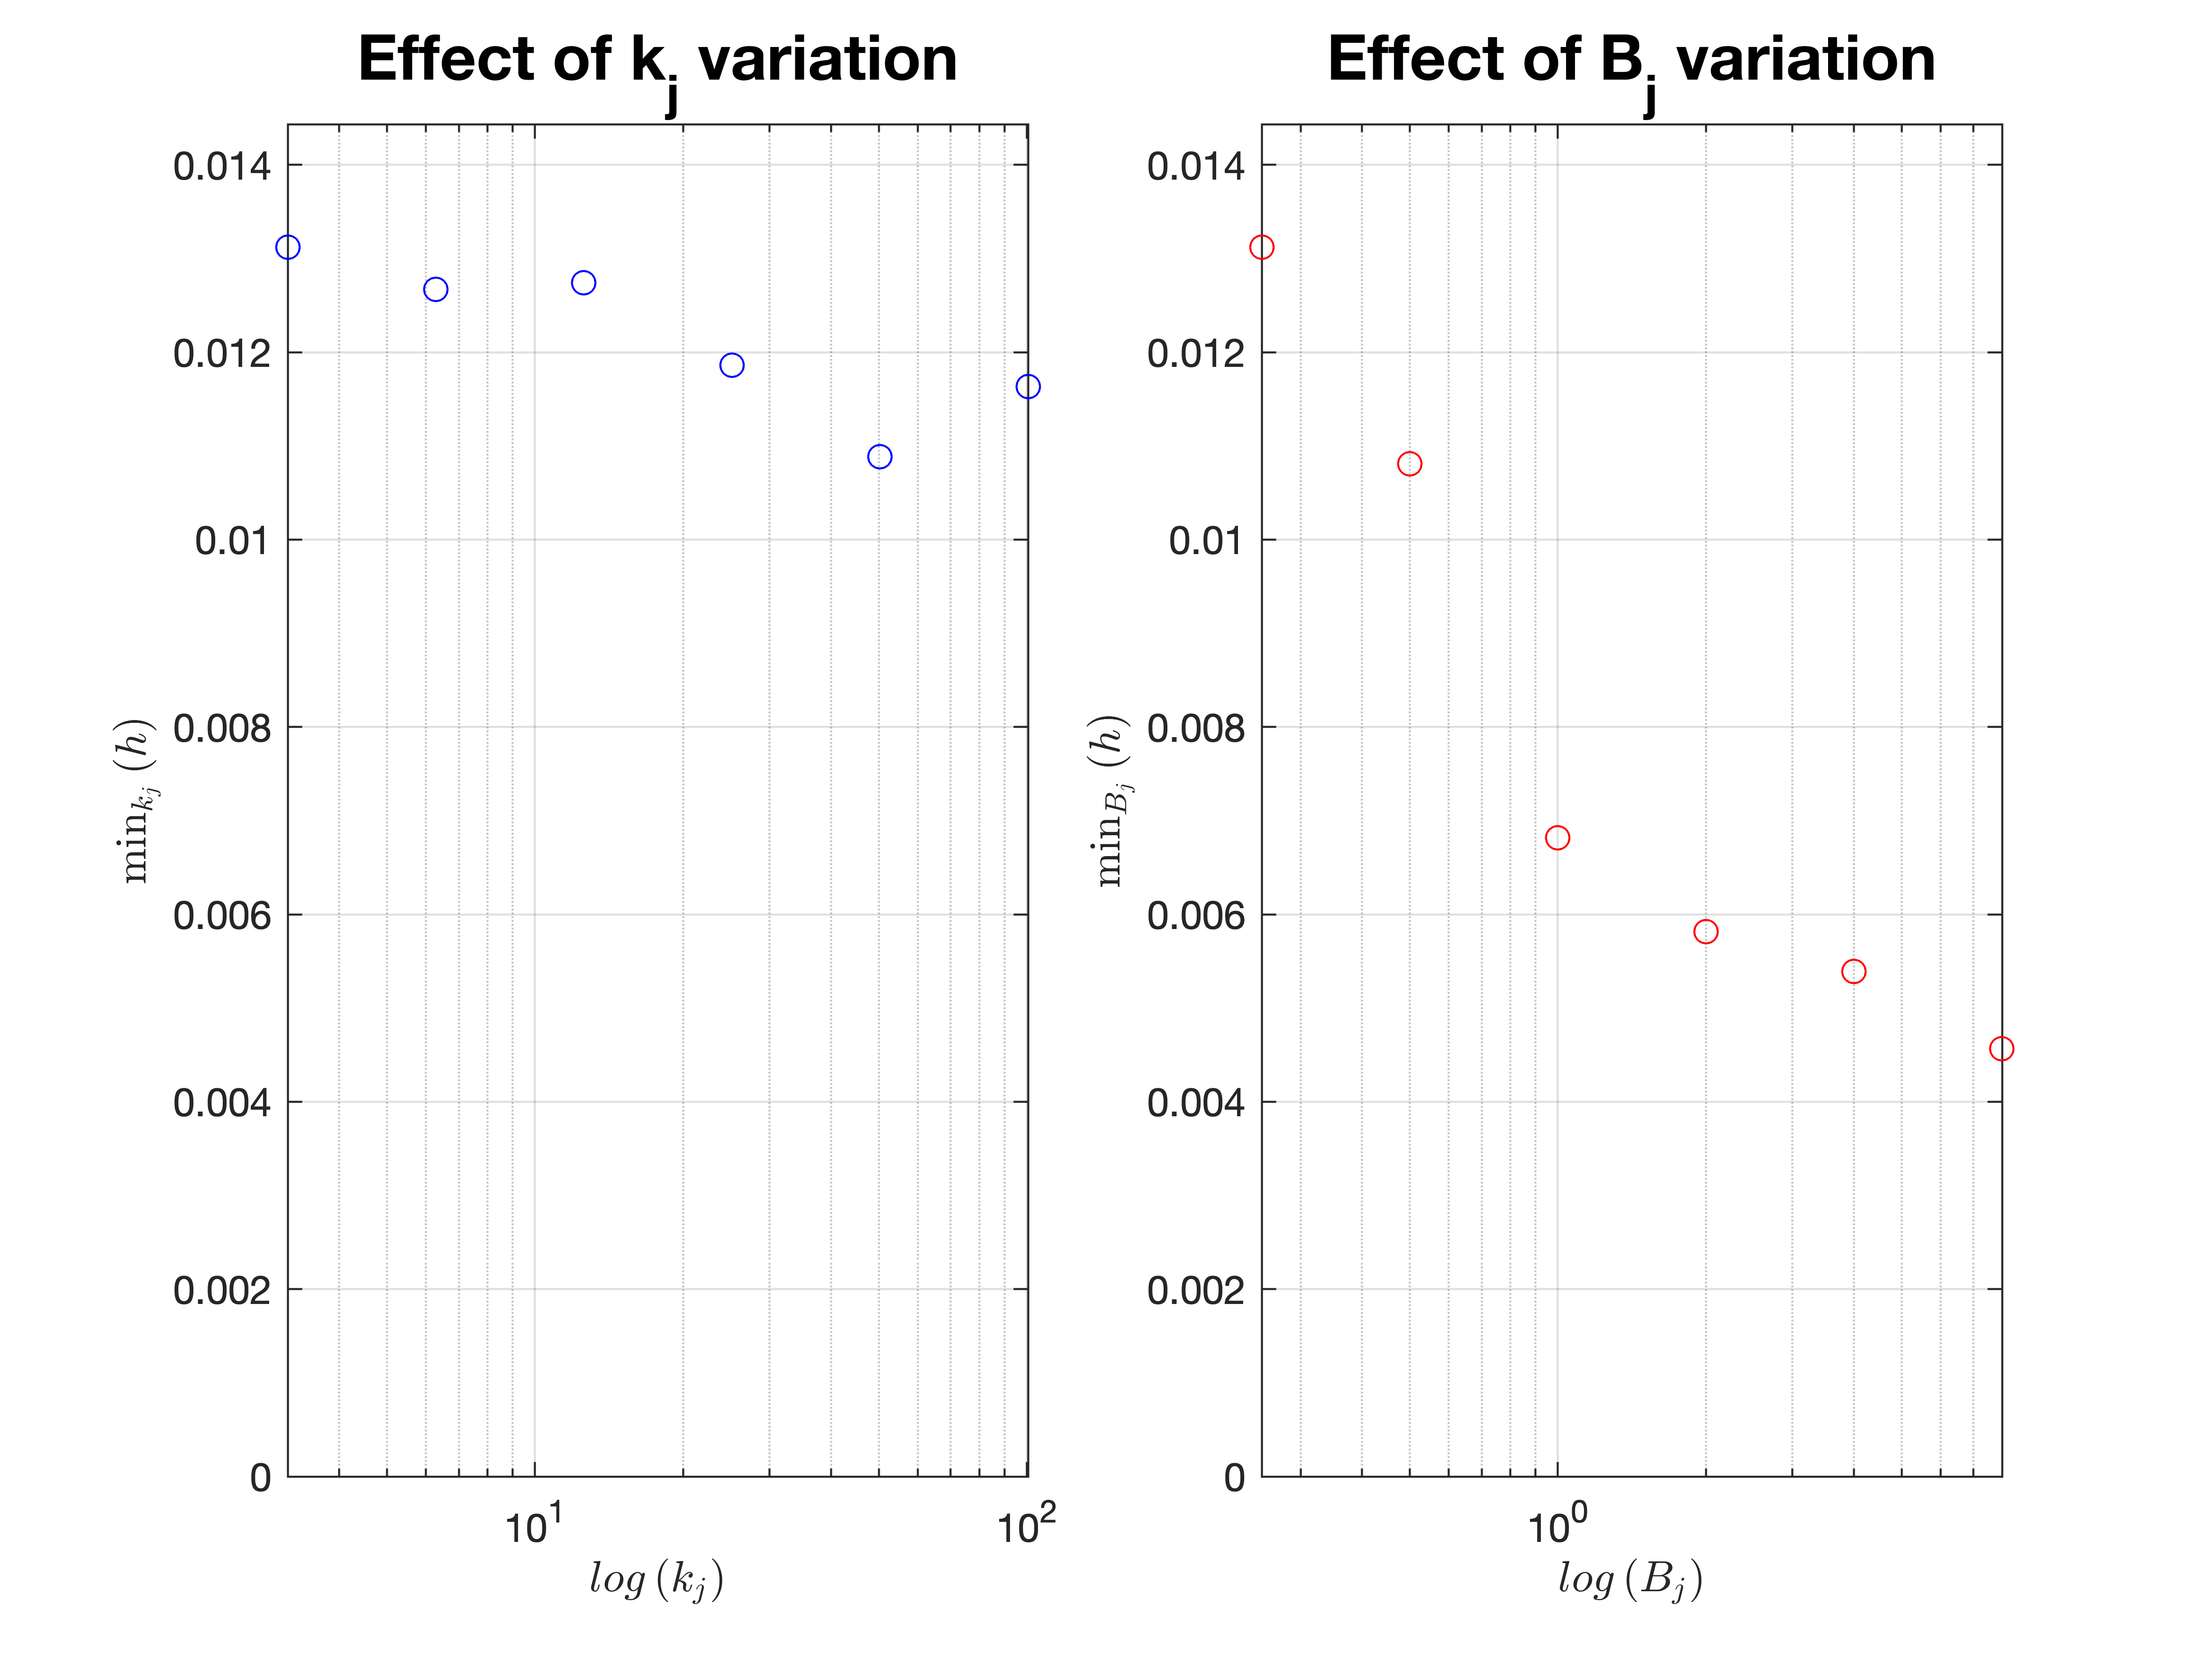
\includegraphics[width=1.0\textwidth]{fig_effect_on_minh_kj_Bj}	
	\caption{\label{fig:effect_Bj_kj_minh}  In this plot we
		examine the effect of varying (individually) the parameters $k_j$ and $B_j$ on $\min{h}$ during a simulation. The parameters are defined in (\ref{eq:second_parameter_set}). }
\end{figure}



\bibliographystyle{alpha}
\bibliography{apostfd,apostfd_bibdesk}
\end{document}